\documentclass[11pt,a4paper]{article}

\usepackage[utf8]{inputenc}
\usepackage[spanish,mexico]{babel}

\usepackage{amsmath, amssymb, amsthm}
\usepackage{mathrsfs}
\usepackage{appendix}
%\usepackage{minted}	

%pdflatex -synctex=1 -interaction=nonstopmode --shell-escape %.tex


\usepackage{hyperref}
\usepackage{captdef}

\usepackage{psfrag}
\usepackage{graphicx}
%\usepackage{subfig}
\usepackage{color}
\usepackage{multicol} 

%\usepackage{fancyhdr}
%\pagestyle{fancy}
%\fancyhf{}


\usepackage{cancel}
\usepackage[usenames,dvipsnames,svgnames,table]{xcolor}
\usepackage[left=2cm,right=2cm,top=2cm,bottom=2cm]{geometry}
\usepackage{caption}
\usepackage{subcaption}
%\renewcommand{\baselinestretch}{1.5}

\usepackage{hyperref}
%\usepackage[hidelinks]{hyperref} 
\hypersetup{
    colorlinks=true,
    linkcolor=blue,
    filecolor=magenta,      
    urlcolor=cyan,
    }

\begin{document}
\thispagestyle{empty}

\includegraphics[height=3.5cm]{escudoCiencias.pdf}
\vspace{-3.8cm}
\begin{flushright}
\hspace{4cm}
{\Large\textbf{Sobre los sistemas lineales y los no lineales}\\
Proyecto de Tesis}
\vspace{0.3cm}\\
\begin{large}Autor: Rodrigo Vega Vilchis.\end{large}\\
\begin{footnotesize}
Correo: rockdrigo6@ciencias.unam.mx\\
\hspace{2.05cm}{\color{white}.}\\
\end{footnotesize}
\vspace{0.1cm}
\begin{large}
Fecha: 06 Abril, 2024\end{large}\\
\end{flushright}
%\vspace{.4cm}
 \hrule height1pt\vspace{.5cm}

\begin{abstract}
hola
\end{abstract} 

\section{Introducción}

En el primer pasaje de esta serie se estuvo revisando la información elemental de los sistemas lineales y no lineales para poder construir la base del proyecto de tesis. Las conclusiones más rescatables son las siguientes: Los sistemas puede ser estables o inestables, en el caso de los sistemas lineales bastará con mostrar que los eigenvalores de la matriz de interacciones asociada el sistema, tienen eigenvalores con parte real negativa; siendo el sistema lineal de la forma
$$\frac{dx_i}{dt}=\sum_j \alpha_{ij}x_j=A\vec{x}$$
donde $\alpha_{ij}$ son los coeficientes de la matriz de interacciones y $x_j$ son los elementos de un vector n-dimensional. La estabilidad también es conocida por puntos críticos en donde convergen todas las soluciones del sistema,  a estos se les conoce como \textit{atractores}. Por el contrario, los puntos de los que divergen las soluciones del sistema se les conoce como fuentes. Otra conclusión destacable del primer pasaje fue acerca de los sistemas no lineales; estos sistemas a diferencia de los anteriores no tienen fácil acceso a soluciones analíticas y se requiere de otro tipo de análisis para su tratamiento. El sistema que estamos centrados es el de Lotka Volterra de competencia dada por las ecuaciones
\begin{equation}\label{eq:sisLK}
\frac{dx_i}{dt}=r_ix_i\left (1-\frac{\sum_j \alpha_{ij}x_j}{K_i}\right )
\end{equation}
Hay que mencionar que este sistema esta basado sobre el modelo logístico de las ecuaciones no lineales solo que un poquito más sofisticado. Este sistema también posee una matriz de interacciones solo que no es la misma que en el caso anterior. Esta matriz de interacciones representa la interacción de la especie $j$ con la especie $i$\footnote{porque en principio $(\alpha_{ij})$ es una matriz aleatoria y el plan es poder meter aquí varios modelos de red para poder investigar la dinámica.} y de acuerdo al coeficiente $\alpha_{ij}$ se verá que tanto afecta la interacción de la $j$ a la $i$. Estos tipos de sistemas no poseen una solución analítica\footnote{al menos no una que yo conozca.} por lo que se opta por escoger a integradores numéricos para que nos develen el tipo de interacciones que presentan.\\
\\
La matriz de interacciones $(\alpha_{ij})$ en este primer alcance esta modelada por una red aleatoria que depende de dos parámetros: $N$ número de especies y una probabilidad de conexión $p$. A este tipo de modelo se le conoce como modelo de red aleatoria propuesta por Erdös-Rényi. Se sabe que la distribución de la matriz aleatoria esta dada por una distribución binomial, pero por ahora no tocaremos ese tema a profundidad. Las entradas de la matriz son números aleatorios que estan definidos por una distribución normal dada por cierta $\sigma$ y centrada en cero.

\section{Estabilidad en sistemas no lineales}

Con todos estos elementos se concluyeron varias cosas. En primer lugar, los coeficientes negativos de esta matriz de interacciones dan lugar a la cooperación entre especies lo que conlleva a la coexistencia de las mismas traducida en la estabilidad del sistema. Por el contrario, los coeficientes positivos dan lugar a la competencia y normalmente genera extinción en las especies pero. En segundo lugar, también depende mucho de la "fuerza" de las interacciones para que el sistema se encuentre estable o inestable, entre menos "débiles" sean esas interacciones, la probabilidad de estabilidad aumenta. En tercer y cuatro lugar, la estabilidad depende sustancialmente del tamaño de la red, entre más grande sea la red es cada vez más complejo y más probable de que el sistema sea inestable (aunque $\sigma<1$ pueda mitigar dichos efectos); la probabilidad también es factor influyente para que el sistema sea estable o inestable. La probabilidad define la cantidad de interacciones de la red, una probabilidad "alta" de conexión define redes con muchos más enlaces que una probabilidad baja.
\begin{figure}[h!]
        \centering
        \begin{subfigure}[h]{0.5\textwidth} 
            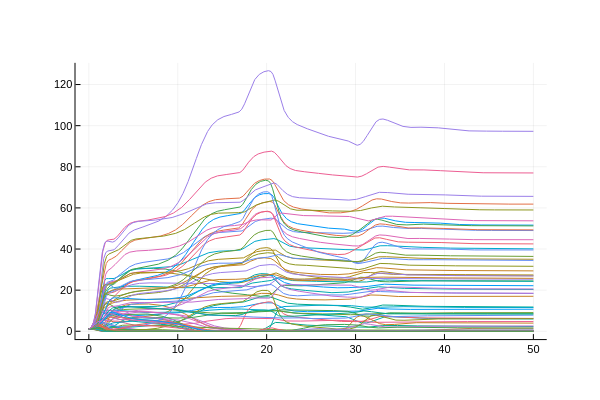
\includegraphics[width=\textwidth]{/home/rogve98/Documentos/Tesis/Tesis/Código/Imagenes/Sistema estable 100}
            \caption{Modelo estable de 100 especies con interacciones gobernadas por números aleatorios de una distribución normal centrada en cero con $\sigma=0.2$}
            \label{fig:Sistema}
        \end{subfigure} 
        \hfill 
        \begin{subfigure}[h]{0.49\textwidth} 
            \includegraphics[width=\textwidth]{/home/rogve98/Documentos/Tesis/Tesis/Código/Imagenes/transición 02-50}
            \caption{Transición de fase para un conjunto de 50 probabilidades entre 0 y 1 con interacciones dadas por números aleatorios de una distribución normal centrada en cero y $\sigma=0.2$}
            \label{fig:transicion}
        \end{subfigure}
        \caption{Estabilidad del sistema \ref{eq:sisLK}}
\end{figure}

Analizando la estabilidad de \ref{fig:Sistema} notamos que existe un punto crítico atractor n-dimensional, es decir, un vector de 100 entradas. La matriz de interacciones de este sistema es de 100 especies, con una probabilidad de $p=0.2$ y con $\sigma=0.2$. El resultado fue la coexistencia de las especies en ese punto atractor. Se recupera el punto atractor para poder sustituirlo en el jacobiano del sistema y de esta manera poder conocer los eigenvalores del sistema, mismos que deben ser negativos para comprobar la relación de los eigenvalores con parte real negativa con la estabilidad del sistema. El resultado es el siguiente
\begin{figure}[h!]
\centering
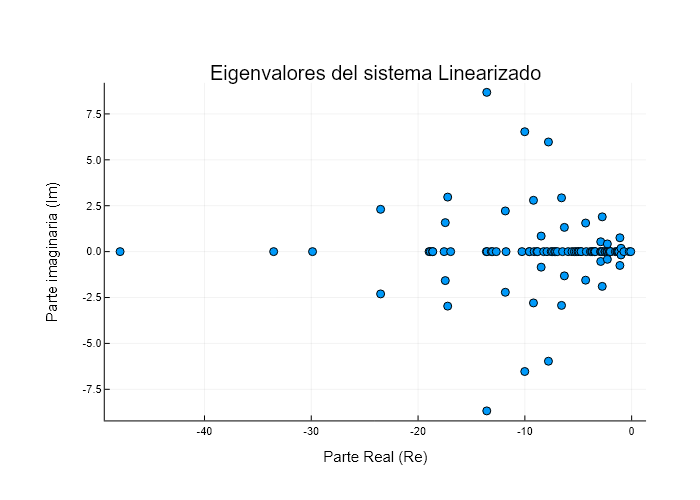
\includegraphics[scale=0.35]{/home/rogve98/Documentos/Tesis/Tesis/Código/Imagenes/Eigenvalores}
\caption{Eigenvalores del sistema \ref{eq:sisLK} de 100 especies, con $p=0.2$ y $\sigma=0.2$. Todos los eigenvalores tienen parte real negativa.}
\end{figure}
 
\end{document}